\section{Reproducible Test Environment}\label{sec:reproducible-test-tenvironment}

This section describes the implementation of the reproducible test environment
as introduced in the concepts chapter~\ref{subsec:reproducible-test-environment-concept}
and specified in the according milestone~\ref{subsubsec:milestone-test-environment}.
The \mintinline{bash}{virtual_enterprise_network_lab.clab.yaml} described in the last subsection~\ref{subsec:contairlab-topology-yaml}
fully describes, specifies and implements the reproducible test environment as required for testing and evaluation.

\subsection{Network Topology}\label{subsec:test-network-topology}

The network topology shown in Figure~\ref{fig:virtual-test-environments} illustrates the IP addressing scheme and the interconnections between the individual components.

The \mintinline{bash}{external} node represents an external attacker interacting with the network from the \gls{WAN}.
The \mintinline{bash}{nsak} container can be deployed in different network segments, enabling the simulation of various attacker positions and reconnaissance scenarios.

\begin{figure}[H]
	\centering
	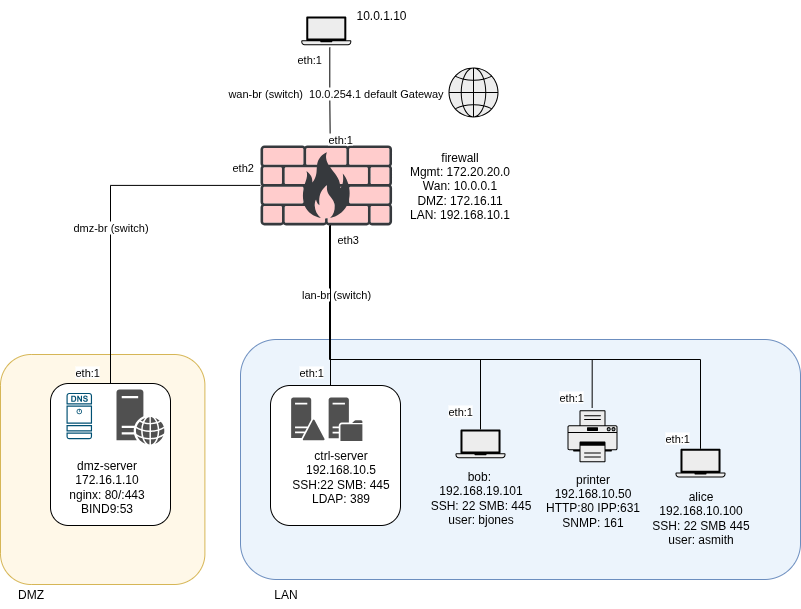
\includegraphics[width=0.8\linewidth]{../assets/diagrams/virtual-environments/virtual-environments.drawio}
	\caption{topology-test-environment}
	\label{fig:virtual-test-environments}
\end{figure}


\subsection{DMZ-Server}\label{subsec:reproducible-test-environment-dmz-server}

To evaluate reconnaissance scenarios, common services must run on endpoints.

\gls{BIND} is a complete implementation of the \gls{DNS} protocol that can be configured through the \mintinline{bash}|named.conf| file as an authoritative name server and resolver.

In the test lab illustrated in~\ref{fig:virtual-test-environments}, the functionality of the web server and \gls{DNS} server was combined for simplicity.

During the \gls{DMZ}-server container build process, a setup shell script is executed.

In the first part, the authoritative \gls{BIND} \mintinline{bash}|named.conf| file, \gls{DNS} options, and master zones for forward and reverse lookups are created.

In the forward zone, domain names map to IP addresses, while in the reverse zone, IP addresses map to domain names~\ref{lst:containerlab-topology-yaml-dmz}.

\begin{figure}[H]
    \centering
    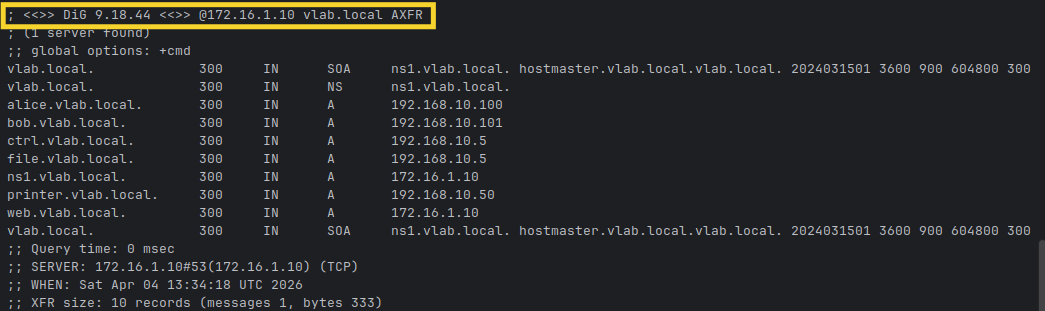
\includegraphics[width=1.0\linewidth]{../assets/screenshots/v-lab/authoritative-zone-transfer-snippet}
    \caption{Authoritative Zone Transfer Snippet}
    \label{fig:authoritative-zone-transfer-snippet}
\end{figure}

The output of a full zone transfer illustrated in figure~\ref{fig:authoritative-zone-transfer-snippet} displays the resolved IP addresses and domain names.
In our test environment, the restriction of \gls{AXFR} requests to only trustworthy IPs is intentionally omitted; the devices are deliberately left unhardened.

In the second part, a minimal \gls{Nginx} web server with \gls{HTTP} and \gls{HTTPS} support is created.
Like in real setups, \gls{HTTP} traffic on port 80 is redirected to \gls{HTTPS} on port 443.
To provide an artifact for reconnaissance purposes, a file named \mintinline{bash}|{secret.txt} containing sensitive data is placed on the server.|

The \gls{LAN} zone of the network, consists of 4 devices.

\subsection{Domain Control and File Server}\label{subsec:ctrl-server}

The internal server, reachable at 192.168.10.5, combines the role of domain controller and file server into a single node.

It exposes \gls{SSH} on port 22, \gls{SMB} on ports 139 and 445, and \gls{LDAP} on port 389.

The \gls{LDAP} service is intentionally misconfigured to permit anonymous read access to the entire \mintinline{bash}|dc=lab,dc=local| directory tree, exposing user accounts and group memberships without authentication.

The \gls{SMB} service provides three shares: \mintinline{bash}|public| is readable without credentials, while \mintinline{bash}|finance| and \mintinline{bash}|it| require valid user accounts.

Sensitive files such as payroll exports and budget summaries are placed in the restricted shares as intentional post-exploitation artifacts~\ref{lst:containerlab-topology-yaml-ctrl-server}.

\subsection{Workstations}\label{subsec:workstations}

Two workstations reside on the \gls{LAN} segment: Alice at 192.168.10.100, assigned to the Finance department, and Bob at 192.168.10.101, assigned to the IT department.

Both nodes expose \gls{SSH} on port 22 and \gls{SMB} on port 445, and both \gls{SSH} banners intentionally disclose the organization name.

On Alice, the home directory of user \mintinline{bash}|asmith| contains a confidential finance report and a drive mapping file that reveals the path to the central file share on the domain server.

On Bob, the home directory of user \mintinline{bash}|bjones| contains a scripts directory with a host inventory that lists all internal IP addresses and their respective roles~\ref{lst:containerlab-topology-yaml-alice}\ref{lst:containerlab-topology-yaml-bob}.

\subsection{Printer}\label{subsec:reproducible-test-environment-printer}

The printer service, reachable at 192.168.10.50, provides two different interfaces.
The first web interface is administrative and is available on port 80.
It shows internal printer metadata, such as device name and contact information.
The printer version is intentionally disclosed in this admin view.
The second interface, a \gls{REST API}, listens on port 631 at the \mintinline{bash}| {/jobs}| endpoint, where it displays a predefined list of print jobs.
All printer requests are logged in \\ \mintinline{bash}|{/var/logs/printer_sim_logs}| inside the container~\ref{lst:containerlab-topology-yaml-printer}.

\subsection{Introduced Vulnerabilities}\label{subsec:introduced-vulnerabilities}

For reconnaissance purposes, several vulnerabilities and flaws were introduced,
which are partly mentioned in the previous sections and are presented in detail in Listing~\ref{lst:containerlab-topology-yaml-overview}.
These flaws are necessary to compare the results of the larger and smaller models as well as the implemented vs the \gls{AI} enhanced scenarios.

\subsection{\gls{Containerlab} \mintinline{bash}{virtual_enterprise_network_lab.clab.yaml}}\label{subsec:contairlab-topology-yaml}

Listings~\ref{lst:containerlab-topology-yaml-overview},
~\ref{lst:containerlab-topology-yaml-network},
~\ref{lst:containerlab-topology-yaml-firewall},
~\ref{lst:containerlab-topology-yaml-dmz},
~\ref{lst:containerlab-topology-yaml-ctrl-server},
~\ref{lst:containerlab-topology-yaml-alice},
~\ref{lst:containerlab-topology-yaml-bob},
~\ref{lst:containerlab-topology-yaml-printer},
~\ref{lst:containerlab-topology-yaml-nsak},
~\ref{lst:containerlab-topology-yaml-links},
in the appendix are showing the \gls{Containerlab} \mintinline{bash}{virtual_enterprise_network_lab.clab.yaml} file.
The nodes are representing hosts as \glspl{OCI-Container},
connected with virtual ethernet links to the bridge, which acts as a multi-port switch.
For simplicity, we decided to use bash scripts to configure and start the services,
instead of building dedicated containers for all hosts.

Together, these nodes form a deliberately unhardened network, containing a range of misconfigured services,
providing a realistic target for evaluating reconnaissance scenarios.
